\documentclass[10pt,border=1pt]{standalone}
\usepackage[T1]{fontenc}
\usepackage{mathpazo}
\usepackage{amsmath,amssymb}
\usepackage{xcolor}
\usepackage{pgfplots}
\pgfplotsset{compat=1.18}
\usetikzlibrary{shapes.geometric,positioning,arrows.meta,calc}
\definecolor{okorange}{HTML}{E69F00}
\definecolor{oksky}{HTML}{56B4E9}
\definecolor{okgreen}{HTML}{009E73}
\definecolor{okblue}{HTML}{0072B2}
\definecolor{okverm}{HTML}{D55E00}
\definecolor{okpurple}{HTML}{CC79A7}
\colorlet{accent}{okverm}
\pgfplotsset{
  safenest/.style={
    tick label style={font=\footnotesize},
    label style={font=\small},
    title style={font=\small, align=left},
    legend style={font=\footnotesize, draw=none, fill=none, cells={anchor=west}},
    grid style={black!12, line width=0.3pt},
    axis line style={black!70, line width=0.4pt},
    tick style={black!70, line width=0.4pt},
    axis lines*=left,
  },
}
\newlength{\figwidth}
\tikzset{every node/.append style={execute at begin node={\hyphenpenalty=10000\exhyphenpenalty=10000\relax}}}
\setlength{\figwidth}{18.47cm}
\begin{document}
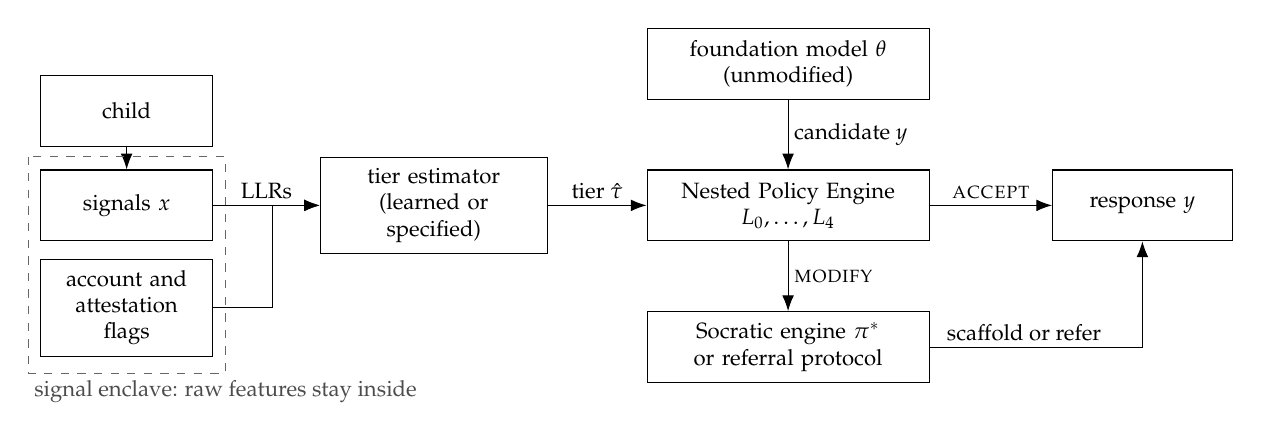
\begin{tikzpicture}[
  box/.style={draw, thin, rectangle, align=center, inner sep=4pt,
              minimum height=9mm, font=\footnotesize},
  ar/.style={-{Latex[length=2mm]}, thin},
  lab/.style={font=\footnotesize, inner sep=2pt},
]
\node[box, text width=19mm] (c)  at (0.7,1.55) {child};
\node[box, text width=19mm] (s)  at (0.7,0.35) {signals $x$};
\node[box, text width=19mm] (dv) at (0.7,-0.95) {account and\\attestation flags};
\node[box, text width=26mm] (est) at (4.6,0.35) {tier estimator\\(learned or specified)};
\node[box, text width=33mm] (pol) at (9.1,0.35) {Nested Policy Engine\\$L_0,\ldots,L_4$};
\node[box, text width=33mm] (llm) at (9.1,2.15) {foundation model $\theta$\\(unmodified)};
\node[box, text width=33mm] (soc) at (9.1,-1.45) {Socratic engine $\pi^{*}$\\or referral protocol};
\node[box, text width=20mm] (out) at (13.6,0.35) {response $y$};
\draw[ar] (c) -- (s);
\draw[ar] (s) -- node[lab, above] {LLRs} (est);
\draw[ar] (dv.east) -- ++(0.75,0) |- (est.west);
\draw[ar] (est) -- node[lab, above] {tier $\hat{\tau}$} (pol);
\draw[ar] (llm) -- node[lab, right] {candidate $y$} (pol);
\draw[ar] (pol) -- node[lab, right] {\textsc{modify}} (soc);
\draw[ar] (pol) -- node[lab, above] {\textsc{accept}} (out);
\draw[ar] (soc.east) -| (out.south);
\node[lab, anchor=south] at ($(soc.east)+(1.2,0)$) {scaffold or refer};
\draw[dashed, thin, black!60] (-0.55,0.97) rectangle (1.95,-1.78);
\node[lab, anchor=north west, text=black!70] at (-0.55,-1.8)
  {signal enclave: raw features stay inside};
\end{tikzpicture}
\end{document}
